\documentclass[10pt,a4paper]{report}
\usepackage[utf8]{inputenc}
\usepackage[francais]{babel}
\usepackage[T1]{fontenc}
\usepackage{amsmath}
\usepackage{amsfonts}
\usepackage{amssymb}
\usepackage{pdfpages}
\usepackage[left=1cm,right=1cm,top=1cm,bottom=1cm]{geometry}
\author{Nicolas Lavoie Drapeau \and Alexandre Mathon-Roy \and Luc-Antoine Girardin \and William Tchoudi \and Lionnel Lemogo}
\title{IFT3912 - Développement et maintenance,\\Plan de développement\\Équipe 1}
\begin{document}
\maketitle
\section*{Résumé}
\indent{Le projet consiste à créer une application web, constitué majoritairement d’un serveur http
spécialisé, qui gère des évènements. Chaque évènement et utilisateurs auront leur page propre afin de
consulter leurs informations respectives.}\\[2ex]
\indent{Lorsque la page web est téléchargée, l’application sera en mode de navigation pour utilisateurs
anonymes. Un utilisateur anonyme aura la possibilité de consulter une liste d’évènements à venir,
d’évènements passés et d’évènement annulés ou chercher des évènements à l’aide d’une barre de recherche pour
ultimement avoir la possibilité de s’y inscrire.}\\[2ex]
\indent{Si un utilisateur anonyme crée un compte ou ouvre sa session, l’application entre en mode de
navigation pour utilisateur enregistré. Un tel utilisateur aura toutes les options d’un utilisateur anonyme,
mais avec certaines options en bonus. Par exemple, un utilisateur enregistré pourra modifier son compte,
consulter la liste des évènements où il est inscrit, créer et gérer ses évènements et commenter des
évènements. Évidemment il pourra se déconnecter.}\\[2ex]
\indent{Le logiciel ainsi créer sera utilisable par tous pour tout genre d’évènements, mais il sera conçu à la base pour des évènements sportifs pour les étudiants de l'Université de Montréal. Ainsi, n’importe quel étudiant pourra organiser par exemple une journée de soccer au parc du coin avec leur association étudiante. Par contre, en plus de gens individuels, des entreprises, des organismes ou encore des associations pourront se servir de l’application pour organiser par exemple leur levé de fonds avec une activité de Zumba, des évènements de sensibilisation à l’importance du sport, etc au CEPSUM. L’application devra donc être bien présentée et professionnelle pour l’utilisation par des entreprises, mais également facile à utiliser, facile à comprendre, bref : simple, pour l’utilisation par des gens communs.}\\[2ex]
\indent{Le système devra donc avoir plusieurs interfaces pour gérer des utilisateurs, des évènements et des
 résultats de recherche. Il devra pouvoir stocker l'information, c'est-à-dire la liste d'utilisateurs,
d'évènement, les commentaires, etc, dans un base de données. Le tout devra être gérer dans un site web
convivial dans un affichage adéquat et rapide (de deux à trois secondes de chargement).}\\[2ex]  
\section*{Work Breakdown Structure}
\begin{enumerate}
\item[1.] Analyse des besoins.\\
\begin{enumerate}
\item[1.1] Analyser les fonctions requises.\\
\item[1.2] Définir les besoins des interfaces web.\\
\item[1.3] Développer l'architecture du système web.\\
\item[1.4] Cas d'utilisation.\\
\end{enumerate}
\item[2.] Analyse des risques.\\
\begin{enumerate}
\item[2.1] Identifier et analyser les risques.\\
\item[2.2] Composer le plan d'aversion des risques.\\
\end{enumerate}
\item[3.] Qualité et métriques.\\
\begin{enumerate}
\item[3.1] Définir les métriques du projet.\\
\item[3.2] Définir l'évaluation de qualité du logiciel.\\
\end{enumerate}
\item[4.] Conception.\\
\begin{enumerate}
\item[4.1] Conception des interfaces web.\\
\item[4.2] Conception du pont entre web et le système d'origine.\\
\item[4.3] Conception de l'architecture du projet.\\
\item[4.4] Conception de la fonctionnalité de recherche.\\
\item[4.5] Conception de la base donnée.\\
\end{enumerate}
\item[5.] Implémentation et tests unitaires.\\
\begin{enumerate}
\item[5.1] Coder la base de données.\\
\item[5.2] Coder les interfaces statiques Web et faire des tests unitaires.\\
\item[5.3] Coder la gestion dynamique de la page Web et faire les tests unitaires.\\
\item[5.4] Coder le pont et faire des tests unitaires.\\
\end{enumerate}
\item[6.] Installation et déploiement.\\
\begin{enumerate}
\item[6.1] Installer le serveur web.\\
\item[6.2] Installer la base de données.\\
\item[6.3] Assurer la communication entre le pont, la base de données et le serveur.\\
\item[6.4] Tester le serveur.\\
\item[6.5] Tester le fonctionnement du pont.\\
\end{enumerate}
\end{enumerate}
\section*{Échéancier et assignation des ressources}
\begin{description}
\item[Taille de l'équipe:] 5 membres.
\item[Expert Web:] 2
\item[Expert DB:] 1
\item[Experts java:] 2
\item[Modèle de l'équipe:] décentralisé
\end{description}
\section*{Analyse des risques}
\begin{tabular}{| p{4cm} | p{5cm} | p{3cm} | p{2cm} |}
\hline
\textbf{Risques relié projet}&&&\\
\hline
Nom risque & Description risque & Pourcentage de risque & Impact\\
\hline
Risque de dépasser la date limite. & Les dates d'échéances sont très rarement respectées. & 80\% & 3\\
\hline
Problèmes de disponibilité du personnel. & Certains coéquipiers pourraient être occupés avec d'autre travaux ou encore avoir des problèmes de santé. & 60\% & 2\\
\hline
Risque de bris matériel. & Il est possible que, par exemple, un bris d'ordinateur portable survienne. & 20\% & 2\\
\hline
Problèmes de compétence du personnel. & Il est possible que certains membres de l'équipe aient des problèmes avec certaines tâches. & 50\% & 1\\
\hline
\hline
\textbf{Risques techniques}&&&\\
\hline
Nom risque & Description risque & Pourcentage de risque & Impact\\
\hline
Risque de documentation de mauvaise qualité. & Il est possible que nous ayons des problèmes reliés aux librairies que nous aurons besoin d'utiliser, ce qui pourrait ralentir notre travail. & 85\% & 1\\
\hline
\end{tabular}
\newpage
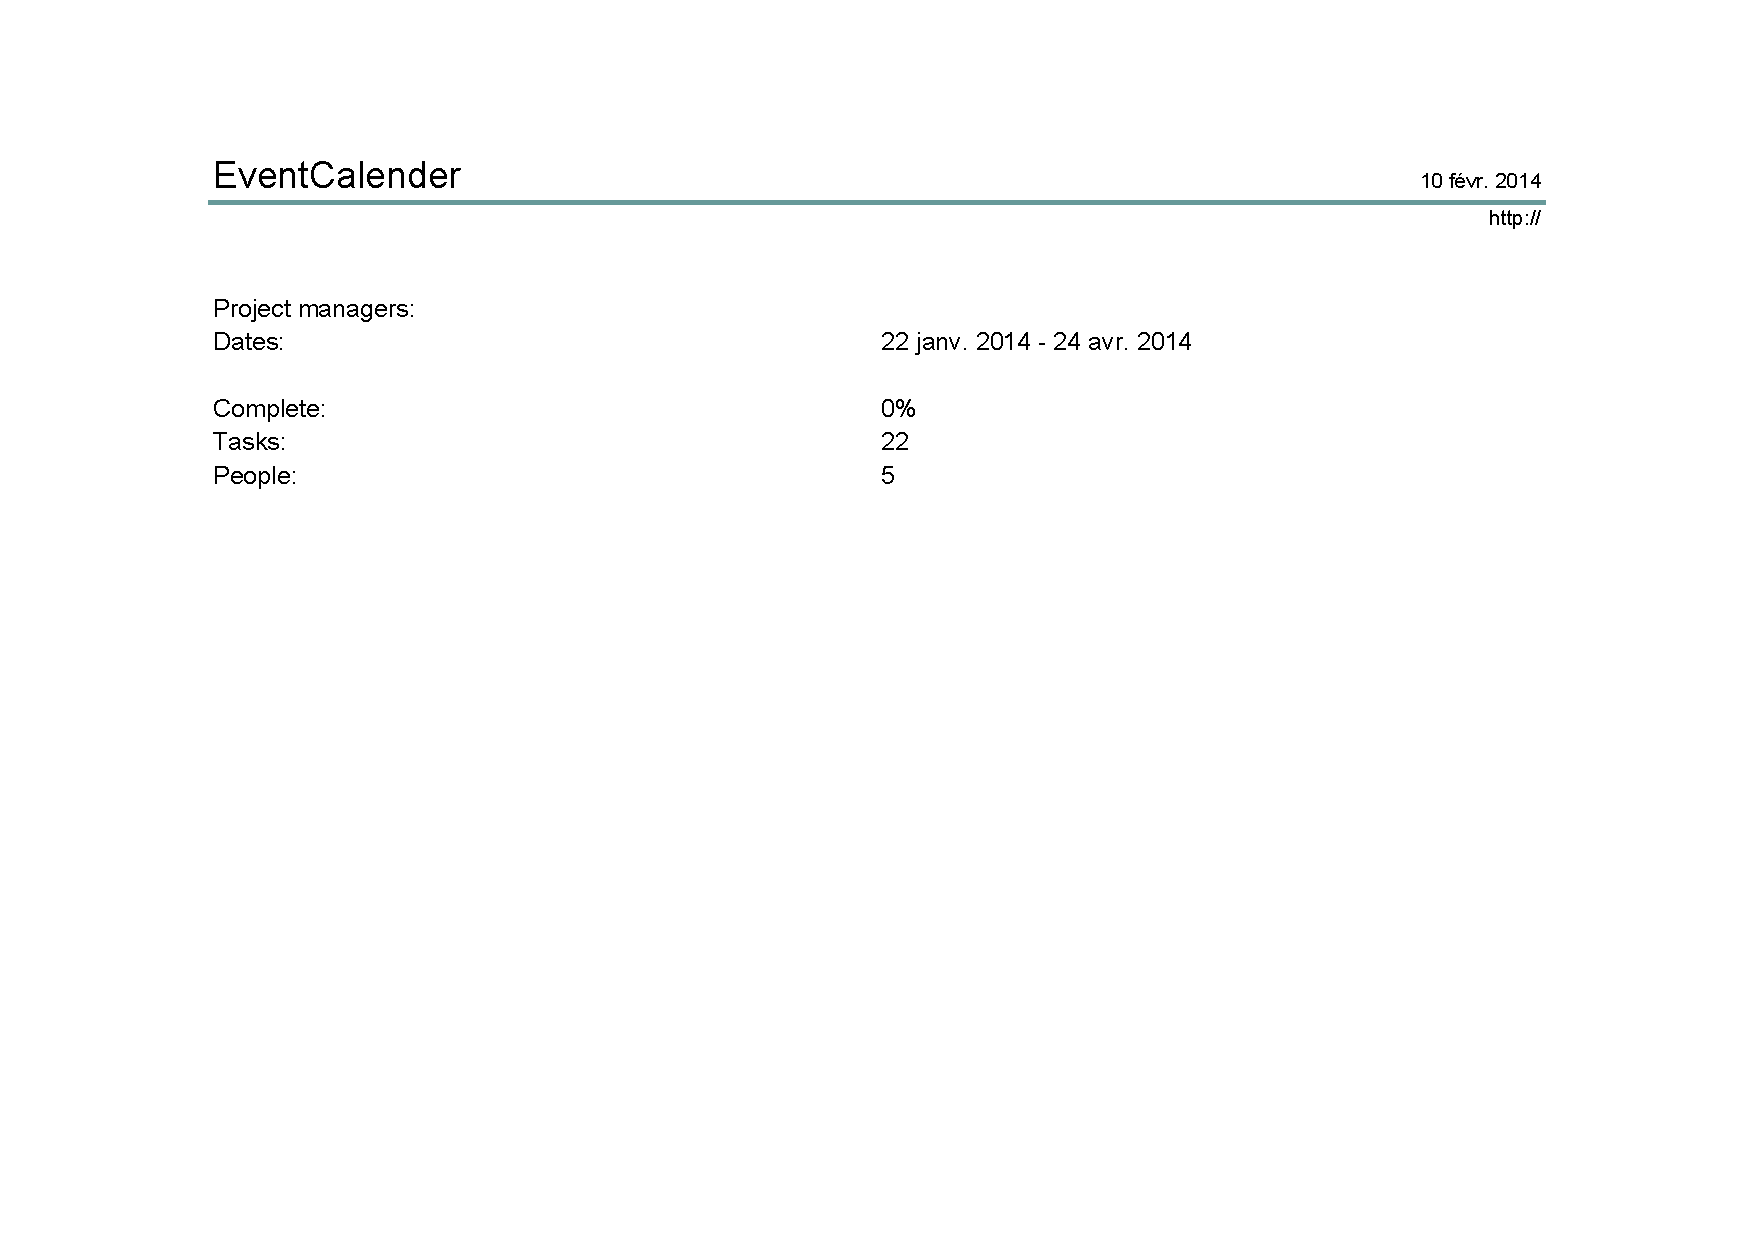
\includepdf[pages={1-3}]{ganttEvent.pdf}
\includepdf[pages={4-5},angle = 90]{ganttEvent.pdf}
\end{document}